\chapter{A Review of B4G/5G Enhancements for Mobility, Latency and NB-I\lowercase{o}T}

\begin{center}
{\large\uppercase{Aloknath De}} 

Samsung R\&D Institute India, Bengaluru

\vskip -6pt

\end{center}

\vskip 2cm




\vfill




\newpage

\begin{multicols}{2}

\section{Introduction}
 
The vision of 5G is to connect multiple devices and provide meaningful services under a common rooftop, enabling the world populace to communicate to each other. It is estimated that industrial Internet of Things (IoT) alone will comprise of more than 25 billion devices by 2025 \cite{art1-key01}-\cite{art1-key02}. All these devices will broadly be cateogrized into three main streams of 5G principles: (1) enhanced Mobile Broadband (eMBB), (2) Ultra Reliable Low Latency Communications (URLLC) and (3) massive Machine-Type Communications (mMTC). They come with their own unique requirements that have to be adhered by the network.

The 5G network supports a large number of UE with varying mobility management needs. This, in turn, has an impact on 5G New Radio (NR) requirements.\break Figure~\ref{chap1-fig01} illustrates the Next Generation Cellular Networks (NGCN) on 3D axis blending requirements, technologies and services. In this article, we describe three techniques, one each for each of the three principles mentioned above. These techniques have been developed primarily by Samsung India researchers in last 12-18 months. They enhance the performance of mobility, latency and narrow-band Internet-of-Things (NB-IoT) machine-to-machine communication. 

\setcounter{figure}{0}
\begin{figure}[H]
\centering
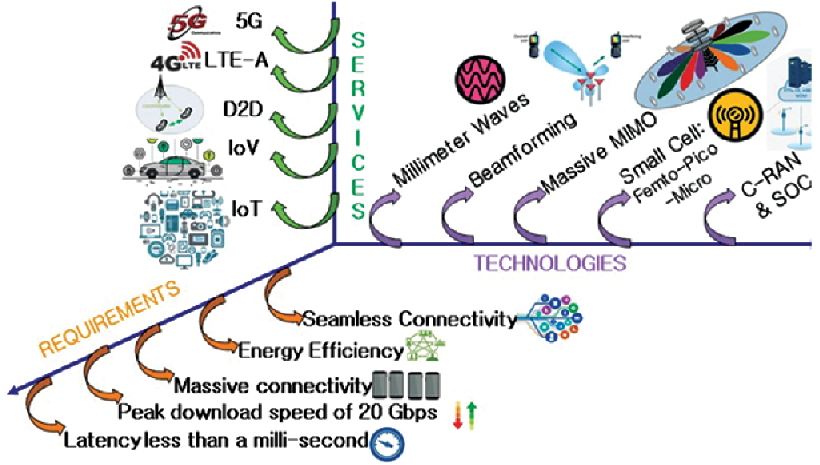
\includegraphics[scale=1.3]{src/Figures/chap1/chap1-fig01.jpg}
\caption{3D axis of Next-Gen Cellular Network}\label{chap1-fig01}
\end{figure}

\section{Maintaining QoS with Varying Degree of Mobility in 5G Network}

\subsection{QoS Variations}

The 5G mobile network incorporates a number of radio technologies; and its requirements are captured in\break Figure~\ref{chap1-fig02}. In such situation, user services necessitate User Equipment (UE) switching between underlying networks to maintain seamless service. This, in turn, leads to overuse of network resources. Frequent switching of UE between different networks leads to congestion in the network. Accordingly, latency and jitter vary depending on the relative position of UE and network components. Maintaining a steady Quality-of-Service (QoS) for the UE under such circumstances is undoubtedly a challenge. In reality, 5G services encounter different mobility scenarios where bigger IoT devices (like AC, Refrigerators) do not require any handovers being in fixed locations, but URLLC portable devices require priority on mobility decision to be able to ensure low latency and secure high bandwidth.

Furthermore, in Ultra dense network, the number of mobility handovers is very high which ultimately results in poor user experience and underutilization of radio resources. In current packet switch mode, mobility parameters are common for all the devices irrespective of their application or use cases which impact the service. QoS differentiation is limited to only data bearer level; but control channel differentiation could improve the differentiated service experience for certain use cases of 5G. As the devices are treated equally in terms of mobility management and different services offered by the network are considered to be undifferentiated, an inefficient spectrum usage and uneven radio resource distribution ensue. The paper \cite{art1-key01} explores how to minimize signaling overhead caused due to different mobility procedures and how to schedule resources properly from the knowledge of UE mobility patterns.

\begin{figure}[H]
\centering
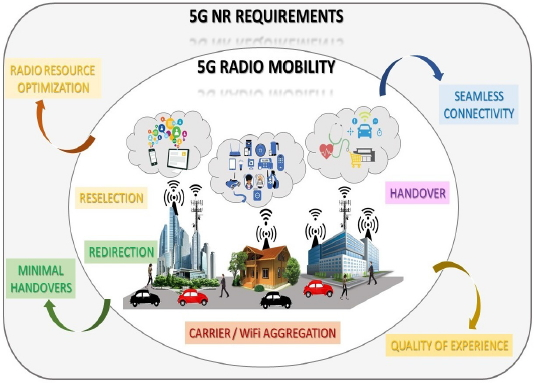
\includegraphics[scale=.75]{src/Figures/chap1/chap1-fig02.jpg}
\caption{5G New Radio (NR) Requirements }\label{chap1-fig02}
\end{figure}


\subsection{Existing Research in Mobility Management}

This section discusses pertinent existing literature in the era of mobility management in 5G. Authors in \cite{art1-key03} define new ways to optimize Software-Defined Network (SDN)-based Distributed Mobility Management (DMM). They rank the nodes based on closeness of nodes to the traffic or have high probability of being on the path of a given UE. These nodes act as anchors for the data plane closer to the nodes instead of using serving gateways of the core network, which leads to  improvement in legacy Long Term Evolution (LTE) handovers.  The paper \cite{art1-key04} presents a network slicing based logical mobility management architecture for 5G. The architecture has slices where each manages its users across differing radio access technologies. The architecture is modular where there is an entity in each slice to handle mobility management. This leads to optimal resource sharing among slices and unify resources of different Radio Access Technologies (RATs).

The paper \cite{art1-key05} describes the mobility level management framework for the connected mode and explains the different level of handover. These levels in connected mode should be dynamically controllable so as to save the network resources and facilitate seamless mobility by reducing the control complexity.  \cite{art1-key06} proposes multiple-level Tracking Area (TA) and Tracking  Area List (TAL) structure which uses UE mobility pattern  and UE density of slices to analyze the location update  frequency and the paging frequency of UE in network slicing.  Based on this structure an embedded Markov chain model is used to find a theoretically optimal TAL configuration of UEs  for slices which reduces the signaling overhead in comparison  to the existing TA strategy and thereby facilitating the mobility  management for network slices.

\subsection{Network Slicing under Varying Degree of Mobility}

Network slicing allows multiple logical network to run on top of a shared physical network. Such slicing in 5G network enables the network to support diverse services along with scalability, flexibility and its requirements. As a consequence, it builds an end-to-end isolated\break network with all virtualized access, transport and core network components for the pertinent end-users. This allows optimal sharing of common physical resources and maximizes the network resource usage. Flexibility provisioned for 5G by network slicing can improve existing mobility management. However, reducing the overhead owing to varying degree of mobility still face many challenges and such overhead can be further optimized with introduction of new scheme.

Devices can be stationary or mobile hence, the network should be able to manage effectively both type of devices. This dynamic scheme tailored for each slice with varying mobility patterns is the novelty introduced in the paper \cite{art1-key01}. The key goal is to curtail the number of handovers thus allowing the network to save the resources for other bandwidth-hungry and latency-intolerant services in the network. The scheme outlines MAS5G (Move Smartly in 5G) that aims to improve the radio mobility procedures  namely initial access (reselection, redirection), location update, handover, carrier/WiFi aggregation. MAS5G Central Mobility Manager (CMM) creates schemas for different network slice based on different UE capabilities and Network Slice Selection Assistance Information (NSSAI). 

This additional information aids differentiated mobility procedures for different class of users based on their use cases, service type, operating mode etc., which will be subset of provisioned services. The paper discusses MAS5G concept for next generation mobile networks. Here are some critical steps:
\begin{itemize}
\itemsep=2pt
\item Different network slice is considered based on three main 5G use cases, i.e. eMBB, URLLC and mMTC. During Network registration, UE shall provide NSSAI and UE capability to Access Mobility Function  (AMF).

\item Based on these two information, the MAS5G CMM  module creates a schema for UE in respective network  slice. With the help of UE capability, if network slice subscribed by subscriber is having skewed features and mobility requirement, CMM creates schema as per the requirements of the particular network slice. 

\item The schemas include mobility parameters in radio at access stratum such as supported features (by a particular slice), RAT-type, service area restrictions, frequency index, preferred neighbor list. Based on different schemas, respective mobility procedures (i.e. Initial Random Access-reselection/redirection, Location Update and handover) are improved for each slice. This helps in reducing the network signaling, reducing radio resource congestion and improving latency. 

\item Based on real time mMTC and eMBB traffic traces, simulation results show that MAS5G is able to curtail the number of handovers, thus, saving the energy at UE significantly, which further helps to boost the QoS.

\end{itemize}

\subsection{Move Smartly in 5G System} 

Mobility management, as highlighted, is a critical function towards maintaining the efficiency of radio network with limited resources and inherent latency. MAS5G scheme identifies different schemas that will govern the mobility of devices in a particular slice. The schemas will narrate: the kind of features a device should support during mobility; RAT-types it can latch to; preferred roaming list; any service area restrictions; allowed frequencies  and preferred neighbor list. The section presents a detailed architecture; message flow and schemas of MAS5G can be studied from original \hbox{paper \cite{art1-key01}.}

The method presents an on-demand and scalable mobility management mechanism under network slicing for customized service scenarios. In existing 5G standards, control plane and the user plane are split and decoupled at the gateway in the core network, and the integrated control functions can reduce control signaling even for a large number of distributed network nodes. However, 5G systems will still face mobility management challenges caused by the potentially ultra-high density of 5G networks combined with high mobility and high density of end devices having different characteristics and requirements in terms of mobility, latency, availability, data rates and reliability. The MAS5G concept is delineated to support seamless user experience with quality, continuity, and scalability based on different UE mobility pattern.

The MAS5G CMM comprises of templates or schemes which are based on network slice specific to service. These schemes are flexible and dynamically updated in runtime. MAS5G CMM is connected to orchestrator and management entities for managing the schemes per slice, it is also connected to 5G core elements like AMF to pass these schemes to 5G NR radio nodes as shown in Figure~\ref{chap1-fig03}. AMF shares UE capabilities and NSSAI with MAS5G CMM through Network Slice Selection Function (NSSF). With these two information, MAS5G CMM provides exclusive mobility schema back to AMF through NSSF. AMF then shares the schema with RAN. Radio nodes prepare specific mobility for serving a UE by segregating radio resources per slice. RAN maps radio resources and parameters based on schemas received per slice, e.g. Random Access Procedure (RACH) parameters, reselection parameters, mobility objects and other measurement events. When one UE opts for multiple network slices simultaneously, MAS5G can manage to pick up any one schema based on priority selection like URLLC over eMBB. However, priority selection and preemption is based on operator’s choice. Through MAS5G network-slicing based mobility, the article explains how to minimize rather optimize the mobility management signaling of each slice hence the control plane resource efficiencies of the 5G mobile network can be achieved. 
\end{multicols}

\begin{figure}[H]
\centering
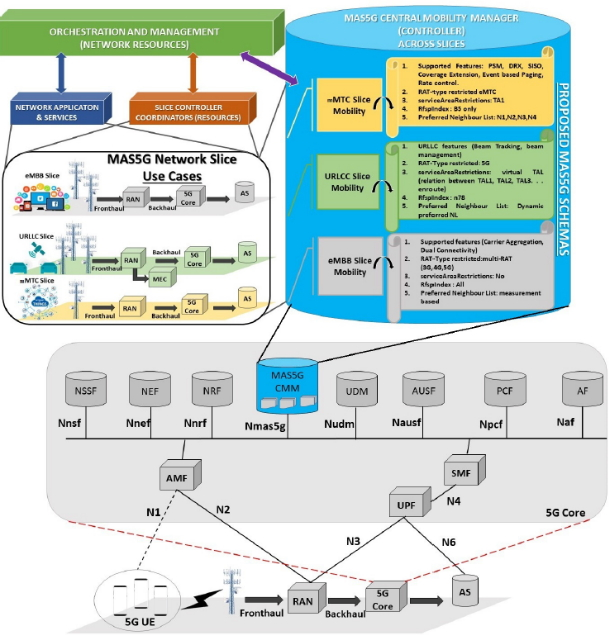
\includegraphics[scale=.8]{src/Figures/chap1/chap1-fig03.jpg}
\caption{MAS5G Architecture}\label{chap1-fig03}
\end{figure}

\begin{multicols}{2}
\section{Optimizing Network Protocol\\ Latencies in Mobile Devices}

\vskip -.2cm

\subsection{Current Research in Protocol Latency Reduction}

Network providers continually improve their infrastructure to support high data rates and reduce infrastructure latencies considerably. Nonetheless, user perceived delay could be reduced further only with\break modifications in transport layer protocols \cite{art1-key07}. There are many researchers working in and around the TCP layer for improving performance on the 5G networks. Some of the research topics are Multi - Core TCP - accelerating device drivers \cite{art1-key08}, Multi - Path TCP - utilizing multiple RATs \cite{art1-key09}, Split - TCP - handling wireless loss \cite{art1-key10}. Also, there are schemes related to adjusting TCP slow start, congestion control and TCP receive window size. These research work are mainly focused on improving throughput of long lived connections. In good number of situations, internet connections are short lived in nature \cite{art1-key11}. For most TCP connections, the content download time is lesser than the socket setup time. The socket setup time creates connectivity overhead and affects overall user experience. Typically, network latency across a wireless network is relatively more than a wired network. The latency of 2G network lies in between 300-1000 ms. For 3G and WiFi network, it lies in between 100-500 ms, whereas for a 4G network, the average latency is less than 100 ms \cite{art1-key12}. Generally one Round Trip Time (RTT) equals to two times of the network latency. Hence the variance of the network latency affects the RTT of the packets. Even though 5G standards set goal to reduce network latency further, the socket setup time takes several RTTs to fetch content from the remote server. Figure~\ref{chap1-fig04} shows the connectivity overhead of protocol stack.

\begin{figure}[H]
\centering
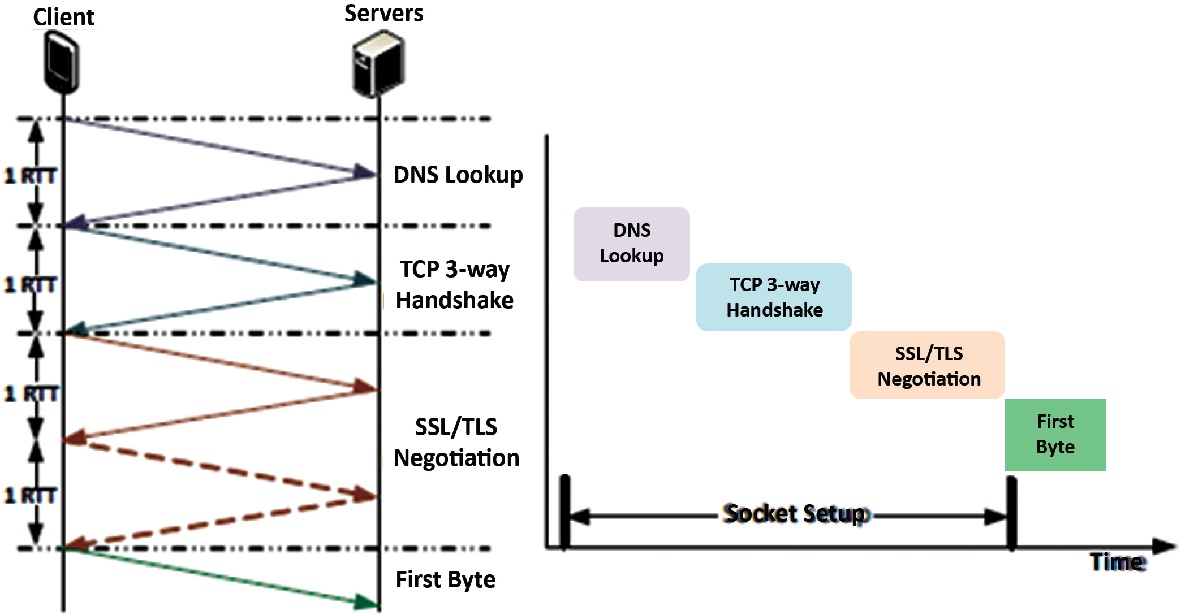
\includegraphics[scale=.9]{src/Figures/chap1/chap1-fig04.jpg}
\caption{Connectivity Overheads of Protocol Stack}\label{chap1-fig04}
\end{figure}

\subsection{System Delay Components}

Let us study the connectivity overheads in protocol stack. Whenever application routes first byte to the server, it first sends request to the operating system for socketsetup. This includes the time of DNS lookup, TCP connect and SSL/TLS negotiation. The socket setup time is unavoidable even though it consumes several RTTs. Web contents hosted across multiple servers are referred with various domain names. The client must perform DNS lookup for resolving domain name to IP address. Usually, the DNS resolution takes at least one RTT. Sometimes, slow responsiveness of DNS server triggers client to send multiple queries, which results in user perceived delay in the client application. After the DNS resolution, client connects to the corresponding server through TCP three-way handshake which consumes additional RTT along with domain name resolution. The RTT of the TCP connect varies from one server to other. It depends upon multiple factors such as type of access network, congestion in the path and server load. In case of busy Internet server, the RTT of the TCP connect increases significantly even in good network conditions. Further in case of secure connections, SSL/TLS certificates are exchanged between client and server. These certificate exchanges add a few more RTTs. Thus cumulative time of DNS Lookup, TCP connect and SSL/TLS certificate exchange along with infrastructure latency considerably affects the user experience.

\subsection{Need of Novel Scheme for Protocol\\ Latency Reduction}

The article \cite{art1-key13} has proposed a novel solution called Layer 4 Accelerator (L4A). It is a client-only software solution, which reduces the latency caused by the network protocols. As the name implies, L4A works on top of Layer 4 of the OSI model. It minimizes connectivity overheads and provides zero RTT socket setup time to the internet applications.

\begin{figure}[H]
\centering
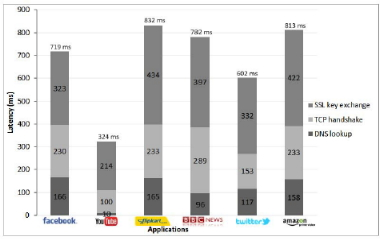
\includegraphics[scale=0.9]{src/Figures/chap1/chap1-fig05.jpg}
\caption{Average socket setup time for popular applications}\label{chap1-fig05}
\end{figure}

\vskip -.2cm

The paper \cite{art1-key13} presents several experiments to analyze connectivity overhead of data protocols; primarily data of 30+ trials has been collected for popular android applications such as YouTube, Facebook, Twitter, popular news and e-commerce applications. Currently, experiments have been conducted in both WiFi, LTE  and other cellular networks and the authors expect to carry out subsequent tests in next-gen networks as they get deployed.  As shown in Figure~\ref{chap1-fig05}, popular applications incur significant delay before sending its first byte to the server. Here are some of the contributing factors \cite{art1-key13} to this delay.

\begin{itemize}
\item  {\bf Minimum TTL value of DNS resource records:} Most of the popular content delivery network (CDN) providers set minimum TTL value in DNS resource records. This helps CDN providers to handle system failover and to distribute load among the servers. These shorter TTL valued DNS queries expire early. This creates additional DNS queries in the network and also increases load on the DNS servers. During experimental analysis, it was found that 80-90$\%$ of shorter TTL valued DNS query responses remain unchanged. On the expiry of DNS query, most of the time-resolver receives unchanged DNS responses for subsequent DNS queries. This causes at least one RTT delay to the requesting application.
\item{\bf DNS cache is not effective in Android:} DNS cache is not completely implemented in Android software stack. There is no dedicated process running on the system for maintaining DNS cache. The Android stack maintains DNS cache based on the smallest TTL (Time-To-Live) value. Even though Android OS evolved over the years, DNS cache is not improved much from Android D (1.6) till the latest version Android N (7.1) \cite{art1-key14}. 
\item {\bf Domain Name Resolution for dual stack (IPv4/IPv6):} In dual stack (IPv4/IPv6) Android devices, DNS lookup takes relatively longer time as compared to IPv4 only capable device, because dual stack device resolves both Type \textit{AAAA} (IPv6) and Type \textit{A} (IPv4) DNS queries in sequence. These cause at least two RTT delay in the dual stacked Android device \cite{art1-key15}. Some OS solves this by implementing IETF proposed algorithm `Happy Eyeballs’ \cite{art1-key16}. As per the algorithm, both Type \textit{AAAA} and Type \textit{A} queries are triggered in parallel and establishes TCP connections immediately. This feature has not been implemented in latest Android version N.
\item{\bf First DNS record used for multiple TCP connections:} Generally CDN DNS servers provide multiple IP addresses to the client application to distribute the load among the content servers. Most of the internet client applications choose first DNS resource record among the multiple resource records. Usually, second and further resource records are ignored by the client application and are not used for successive TCP connections. Even though client application failed to connect first IP address, the other resource records are not used.
\item{\bf TCP backlog queue affects TCP connect time:} In general, each TCP connection establishment should progress through backlog queue of the server. Before receiving any data from the client, first server processes the pending connections from the backlog queue and establishes the connection. This adds queuing delay into initial RTT of the TCP connection.
\item{\bf Secure certificate exchange consumes a few more RTTs:} Once TCP connection is established with the server, secure certificates are exchanged between client and server for making connection secure. This process consumes a few more RTTs before sending first byte to the server. In TLS version 1.2, secure certificate exchange consumes at least two RTTs for securing the connection. The recent version of TLS 1.3 reduced the handshake latency to half \cite{art1-key17}. However, this also requires at least one RTT for secure certificate exchange. To mitigate the above explained problems, L4A solution is implemented in Android and Linux platforms; L4A solution consistently improved application page loading time by 20-30$\%$ on both WiFi and cellular networks.
\end{itemize}

\subsection{Overview of Layer 4 Accelerator (L4A)Method}

\begin{figure}[H]
\centering
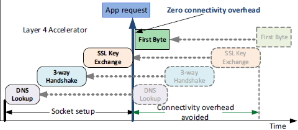
\includegraphics[scale=.9]{src/Figures/chap1/chap1-fig06.jpg}
\caption{Overview of Layer 4 Accelerator operations}\label{chap1-fig06}
\end{figure}

\vskip -.5cm

Layer 4 Accelerator provides cross layer design for optimizing network protocol latencies in mobile devices. The socket setup time causes connectivity overhead in protocol stack which affects the page loading time of the application and impacts the user experience. The socket setup time is unavoidable even though it introduces significant amount of delay for an application. As shown in Figure~\ref{chap1-fig06}, L4A solves this problem by moving socket setup time ahead of application request.

L4A performs DNS lookup, TCP connect and SSL/TLS negotiation in advance and provides zero connectivity overhead to the applications. L4A comprises of three modules, namely, DNS Yielder, TCP Pre-Connector (TPC) and Secure Session Offloader (SSO). As shown in Figure~\ref{chap1-fig07}, L4A is sandwiched between \textit{libc} and application layer. DNS Yielder mainly reduces DNS lookup overhead by pre-resolving domain name in advance and caches the DNS query responses which are frequently requested by the application. DNS Yielder also performs DNS query optimization by analyzing DNS pattern of the application. TCP Pre-Connector avoids TCP three-way handshake latency by connecting to the TCP server ahead of time. Secure Session Offloader (SSO) performs SSL/TLS certificate exchange on behalf of the application and avoids the delay caused by secure certificate exchange.

\begin{figure}[H]
\centering
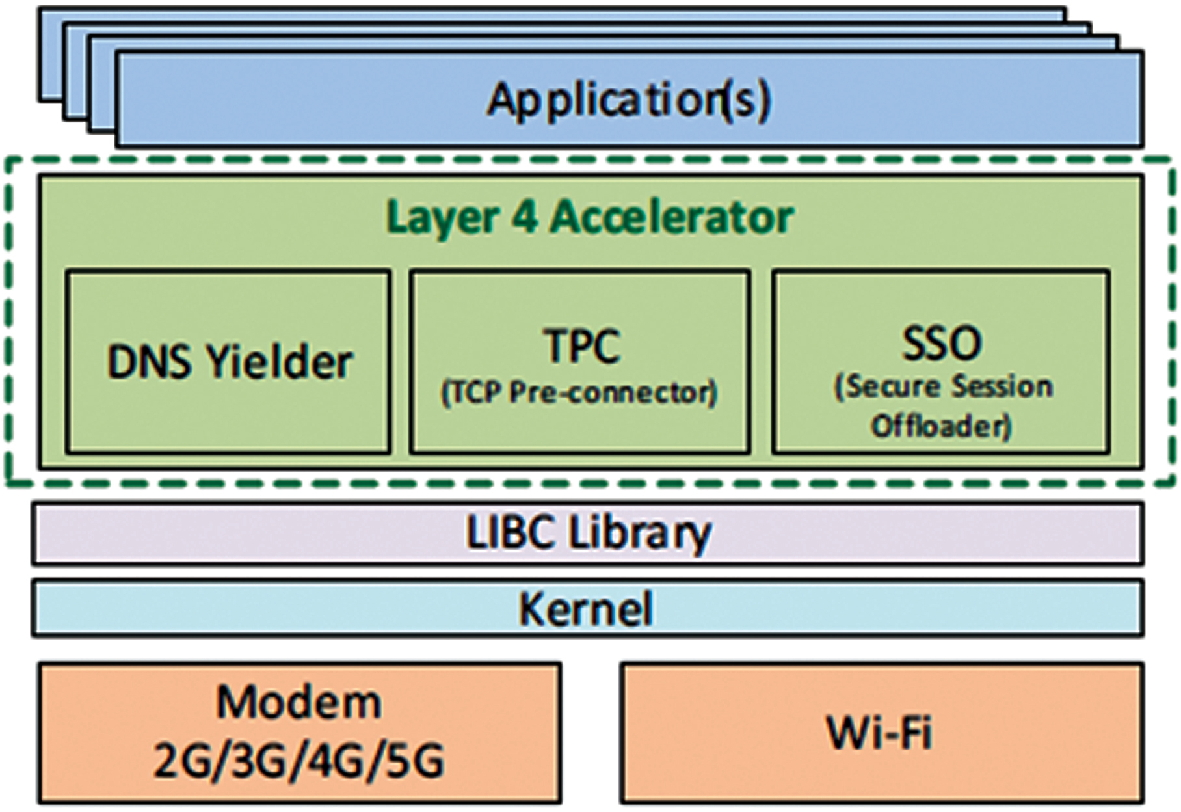
\includegraphics[scale=.9]{src/Figures/chap1/chap1-fig07.jpg}
\caption{Software Architecture of Layer 4 Accelerator}\label{chap1-fig07}
\end{figure}

\subsection{Key Enhancements in Protocol Design}

To solve the connectivity overhead of Internet protocol suite, Google proposed a new data protocol called QUIC which uses UDP as transport layer. QUIC reduces connection latency by providing zero RTT connections to Google applications \cite{art1-key18}. However, it requires changes in both client and server for deployment. TCP evolved over decades and dominated the current Internet protocol suite. Even though Google deploys QUIC in its applications and  servers, it is difficult for all other application to replace TCP. The QUIC protocol is currently being standardized by the IETF QUIC working group \cite{art1-key19}. The other similar proposal called TCP Fast Open (TFO), saves the RTT of the initial connection handshake compared to standard TCP \cite{art1-key20}. Samsung published a patent \cite{art1-key21} for pre-fetching web pages in advance. This idea requires proxy server in middle and is limited to HTTP only. Patent \cite{art1-key22} projects method for reducing network connection latency and navigation latency which also require user interaction as input and are limited to browser applications. L4A is completely different from these earlier works. It does not rely on any user inputs and does not operate specific to applications or protocols. It is a client only and platform independent solution.  L4A is not limited to only HTTP/HTTPS protocols. It supports all application layer protocols like POP3, IMAP, SMTP, etc. L4A is a platform independent solution which is easily deployable in Android and Tizen platforms and can be incorporated in many devices such as Smart phones, Tablets, etc.

Reducing latency across the Internet is of immense value. Measurements and analysis by prominent Internet companies have shown that shaving off a few hundred milliseconds from the time for a transaction can monetarily translate into millions of dollars \cite{art1-key23}. For Amazon, a 100 ms latency penalty implies a 1$\%$ sales loss; for Google, an additional delay of 400 ms in search responses reduces search volume by 0.74$\%$; and for Bing, 500 ms of latency decreases revenue per user by 1.2$\%$. Undercutting a competitor’s latency by as little as 250 ms is considered a competitive advantage in the industry. Even more crucially, these numbers underscore that latency is a key determinant of user experience. Hence, our attempt to reduce initial connection latency using L4A is a positive move towards the new trend in Smart phones and hence it is a value added solution for practical applications. 

\section{Opportunistic Early Decoding for NB-IoT Devices using Link\\ Abstraction}

\subsection{Narrow-Band IoT Operation}

NB-IoT is an IoT solution defined by 3GPP in Release 13 to be deployed on cellular networks to support vast number of low-cost IoT devices with low data rates. IoT devices are expected to be deployed in remote locations and basements with poor signal conditions and the battery also need to last long with an expectancy of 5-10 years without charge \cite{art1-key24}. Hence the key requirements of an NB-IoT device are low power consumption and an extended coverage of 15-20 dB over earlier releases \cite{art1-key25}-\cite{art1-key26}. To support low power consumption and improved battery life in NB-IoT, 3GPP has introduced two new procedures namely power saving mode (PSM) and extended discontinuous reception cycle (eDRX). For increasing the coverage of an NB-IoT device, a new feature called repetitions has been introduced in Rel-13 where the data and the control signals are transmitted repeatedly for a given number of times (N$\scriptsize{\text{Rep}}$). Though Rel-13 eMTC also stands on the similar requirements and features, NB-IoT can be considered as substantially lower cost structure with an operating bandwidth of 180 kHz (1 PRB) supporting layer1 downlink data rates up to 200 kbps \cite{art1-key27} compared to eMTC which operates within a bandwidth of 1.08 MHz (6 PRBs) supporting data rates of $\sim$1 Mbps \cite{art1-key27}.

NB-IoT operates in three different modes: In-band, Guard-band and Stand-alone. In-band uses the PRBs within LTE carrier bandwidth, guard-band uses the unused PRBs within LTE guard bands whereas stand-alone uses the GSM carrier \cite{art1-key25}. Given the NB-IoT bandwidth is very low i.e., 180 KHz (1 PRB) and the largest transport block size (TBS) of downlink data being 680 bits and that of uplink data being 1000 bits \cite{art1-key06} for Rel-13 NB-IoT, it is agreed in 3GPP that the data in NB-IoT will be spread across multiple subframes (N$\scriptsize{\text{SF}}$ ). For NB-IoT downlink, the TB spread across N$\scriptsize{\text{SF}}$ subframes will be transmitted repeatedly for an N$\scriptsize{\text{Rep}}$ repetitions which can take discrete values ranging from 1 to 2048 \cite{art1-key27}. With the introduction of new parameter N$\scriptsize{\text{Rep}}$ in latest 3GPP technologies like MTC, eMTC and NB-IoT, link adaptation method in two dimensions (2-D) has gained interest with N$\scriptsize{\text{Rep}}$ being one of the dimensions. Second dimension for NB-IoT is the transport block size index, ITBS. It is shown that, using 2-D link adaptation method, network is able to allocate the resources efficiently for NB-IoT in uplink in both the dimensions of I$\scriptsize{\text{TBS}}$ and N$\scriptsize{\text{Rep}}$ such that the target BLER (not exceeding 10$\%$) is obtained. Similar method can be adapted for downlink as well. However, the repetition parameter N$\scriptsize{\text{Rep}}$ can be adapted by the network only in discrete levels. 

\subsection{Opportunistic Decode Scheme}

The paper \cite{art1-key28} presents a new decode scheme. Reducing or increasing the assigned N$\scriptsize{\text{Rep}}$ parameter will have a lot of impact in terms of active time of the device due to the finite set of values that can be taken by N$\scriptsize{\text{Rep}}$ as agreed in 3GPP \cite{art1-key27}. For example, if a UE is assigned a resource set I$\scriptsize{\text{TBS}}$=1;N$\scriptsize{\text{Rep}}$=192, it is possible for the UE to successfully decode early at $150^{\scriptsize{\text{th}}}$ repetition level when channel conditions are in favor. Network cannot allocate the next available lower repetition value in this case i.e., 128 at which UE would not be able to decode the data successfully. Also, attempting to decode at the end of 192 repetitions will result in wastage of power at the UE receiver. To avoid power wastage when the channel conditions are in favor, a method of opportunistic early decode (OED) is proposed for NB-IoT devices in downlink. This method helps UE to identify the repetition level at which the downlink data can be successfully decoded opportunistically based on the instantaneous channel conditions. Received Bit Information Rate (RBIR) is chosen as the decoding metric in this method to detect the channel favorable conditions and identify the required repetition level. Unlike the regular modem, once the data is successfully decoded at the identified repetition level, UE can turn off its receiver operations and go to SLEEP mode for the rest of the scheduled repetitions. With this method, we show that the power consumption of an NB-IoT device can be reduced significantly in terms of the active time of the device. 

In NB-IoT system, downlink data is carried by narrowband physical downlink shared channel (NPDSCH). Resource information for the same is carried by DCI format N1 through narrowband physical downlink control channel (NPDCCH) and the feedback of NPDSCH is transmitted in narrowband uplink shared channel (NPUSCH) using format 2 as shown in Figure~\ref{chap1-fig08}. Given the repetitions of NPDSCH varies from 1 to 2048, the device can successfully decode the NPDSCH TB earlier than the scheduled transmission end when the channel conditions are favorable.

\begin{figure}[H]
\centering
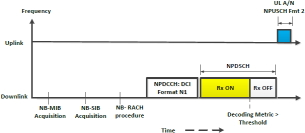
\includegraphics[scale=.9]{src/Figures/chap1/chap1-fig08.jpg}
\caption{OED algorithm implemented in NB-IoT downlink channel, NPDSCH.}\label{chap1-fig08}
\end{figure}

A successful early decode can reduce the power consumption of the device significantly. Attempting to decode at each and every repetition level is one method to check if the TB can be decoded early before the scheduled N$\scriptsize{\text{Rep}}$. But by doing so, the device might end up in consuming more power than the traditional decoding procedure at the end of N$\scriptsize{\text{Rep}}$. Hence a method which checks for the decoding feasibility by predicting the link performance at every repetition level based on instantaneous channel conditions using a metric called decoding metric (D$\scriptsize{\text{m}}$) is required. Figure~\ref{chap1-fig08} shows a scenario where a decoding metric was used at the receiver in an ongoing NPDSCH reception to check the decoding feasibility of the transmitted TB. And once the TB is successfully decoded, UE can ignore the rest of the repetitions to go to SLEEP mode and thus save power.

Link abstraction for regular LTE UEs has been studied well in \cite{art1-key29}. It is a method which predicts the instantaneous fading link performance of a system using the already obtained AWGN channel performance statistics of the same system. It has been shown in \cite{art1-key29} that received bit information rate (RBIR) metric obtained using Mutual Information (MI) - based link abstraction model serves as a good fading insensitive parameter for link performance prediction. Given RBIR is a metric that has one-to-one mapping with the BLER performance of a system independent to channel fading characteristics \cite{art1-key07}, we choose this metric as the decoding metric (D$\scriptsize{\text{m}}$) for NB-IoT downlink. But, obtaining RBIR metric for NB-IoT system can be challenging for two reasons. Firstly, NB-IoT system capable of operating in very low SNR range i.e., below - 10dB, observes high channel estimation error (CEE) at such low SNRs. Hence the MI obtained using post-equalized SNR \cite{art1-key29}-\cite{art1-key30} can be prone to CEE, which needs to be accounted. Second reason is the difference in ratematching procedure of NPDSCH compared to PDSCH in LTE or MPDSCH in eMTC respectively. Unlike LTE/eMTC, NPDSCH in NB-IoT is mapped across multiple subframes (N$\scriptsize{\text{SF}}$) and repeated for N$\scriptsize{\text{Rep}}$ times \cite{art1-key27}. As the RBIR metric is obtained for a TB transmission, it is required that the channel conditions of all N$\scriptsize{\text{SF}}$ subframes need to be considered for obtaining mutual information of every information bit sent in an NPDSCH TB.

\section{Concluding Remarks}

This article reviews three techniques proposed by Samsung India researchers for 4BG/5G systems. 5G is characterized by three key factors: (i) Enhanced Mobile Broadband (eMBB), (2) Ultra-reliable low-latency communication (URLLC) and (3) Massive machine-type communication (mMTC). The first method discusses how QoS could be maintained with varying degree of mobility in 5G network. The second technique discusses optimization of network protocol latencies. The third method highlights how such large-scale system could accommodate narrow-band IoT information.

\vskip -.85cm

\hfill\raisebox{-.1cm}{
\includegraphics[scale=.9]{src/Figures/circledC.eps}}

\begin{thebibliography}{99}
\bibitem{art1-key01} Satish Kumar, Rahul Banerji, Naman Gupta, Suman Kumar, Sukhdeep Singh, Avinash Bhat, Seungil Yoon and Bharat JR Sahu, “MAS5G Move around smartly in 5G” The 7th International Conference on Future Internet of Things and Cloud (FiCloud 2019), Istanbul, 2019.
\bibitem{art1-key02} P Payaswini, D. H Manjaiah, ”Challenges and issues in 4G Networks Mobility Management”, Cornell Univesity arXiv, Feb 2014.
\bibitem{art1-key03} M. Khanfouci, ``Distributed mobility management based on centrality for dense 5G networks,” 2017 European Conference on Networks and Communications (EuCNC), Oulu, 2017, pp. 1-6.
\bibitem{art1-key04} A. Alfoudi, M. Dighriri, A. Otebolaku, R. Pereira and G. Lee, ``Mobility Management Architecture in Different RATs Based Network Slicing,” 2018 32nd International Conference on Advanced Information Networking and Applications Workshops (WAINA), Krakow, 2018, pp. 270-274.
\bibitem{art1-key05} J. Song, T. Yoo and P. J. Song, ``Mobility level management for 5G network,”2016 International Conference on Information and Communication Technology Convergence (ICTC), Jeju, 2016, pp. 940-943.
\bibitem{art1-key06} R. Wen, G. Feng, J. Zhou and S. Qin, ``Mobility Management for Network Slicing Based 5G Networks,” 2018 IEEE 18th International Conference on Communication Technology (ICCT), Chongqing, 2018, pp. 291-296.
\bibitem{art1-key07} A. Singla, B. Chandrasekaran, P. B. Godfrey, and B. Maggs, ``The internet at the speed of light,” in \textit{Proceedings of the 13th ACM Workshop on Hot Topics in Networks,} ser. HotNets-XIII. New York, NY, USA: ACM, 2014, pp. 1:1–1:7. [Online].

 Available: \url{http://doi.acm.org/10.1145/2670518.2673876}

\bibitem{art1-key08} E. Jeong, S. Wood, M. Jamshed, H. Jeong, S. Ihm, D. Han, and K. Park, ``mtcp: a highly scalable user-level tcp stack for multicore systems,” in \textit{11th USENIX Symposium on Networked Systems Design and Implementation (NSDI 14).} Seattle, WA: USENIX Association, 2014, pp. 489–502.
\bibitem{art1-key09} Y.-C. Chen, Y.-s. Lim, R. J. Gibbens, E. M. Nahum, R. Khalili, and D. Towsley, ``A measurement-based study of multipath tcp performance over wireless networks,” in \textit{Proceedings of the 2013 Conference on Internet Measurement Conference,} ser. IMC ’13. New York, NY, USA: ACM, 2013, pp. 455–468.
\bibitem{art1-key10} S. Kopparty, S. V. Krishnamurthy, M. Faloutsos, and S. K. Tripathi, ``Split tcp for mobile ad hoc networks,” in \textit{Global Telecommunications Conference, 2002. GLOBECOM ’02. IEEE,} vol. 1, Nov 2002, pp.138–142 vol.1.
\bibitem{art1-key11} R.Wang et al, ``TCP startup performance in large bandwidth networks,”in IEEE Infocom 2004, vol. 2, March 2004, pp.796-805.
\bibitem{art1-key12} I. Grigorik, ``Mobile Networks: Performance of wireless networks,”in High Performance of Browser Networking, O’Reilly Media, Inc. 2013.
\bibitem{art1-key13} Karthikeyan Arunachalam, Jamsheed Manja Ppallan, Sweta Jaiswal, Rohit Shankar Lingappa, Vikash Balasubramanian and Karthikeyan Subramaniam, “Layer 4 Accelerator (L4A) for optimizing network protocol latencies in mobile devices, “2018 IEEE 20th International Conference on High Performance Computing and Communications (HPCC 2018), Exeter, UK, 2018
\bibitem{art1-key14} “The android open source project,”

 \url{https://android.googlesource.com/platform/bionic/+/android-7.1.1 r46/libc/dns/resolv/res cache.c,} accessed: 2017-07-21

\bibitem{art1-key15} U. Goel, M. Steiner, M. P. Wittie, M. Flack, and S. Ludin, “A case for faster mobile web in cellular ipv6 networks,” \textit{in Proceedings of the 22Nd Annual International Conference on Mobile Computing and Networking,} ser. MobiCom ’16, New York, NY, USA, 2016, pp. 176–188.
\bibitem{art1-key16} D. Wing and A. Yourtchenko, “Happy Eyeballs: Success with Dual-Stack Hosts,” RFC 6555, Tech. Rep. 6555, Apr. 2012. [Online]. 

Available: \url{https://rfc-editor.org/rfc/rfc6555.txt}

\bibitem{art1-key17} A. Langley, N. Modadugu, and B. Moeller, “Transport Layer Security (TLS) False Start,” Internet Requests for Comments, RFC 7918, August 2016. [Online]. 

Available: \url{https://tools.ietf.org/html/rfc7918}

\bibitem{art1-key18} J. Roskind, “QUIC(Quick UDP Internet Connections): Multiplexed Stream Transport Over UDP.” Technical report, Google (2013), Tech.Rep.
\bibitem{art1-key19} “Innovating transport with quic: Design approaches and research challenges,” \textit{IEEE Internet Computing,} vol. 21, no. 2, pp. 72–76, 2017.
\bibitem{art1-key20} S. Radhakrishnan, Y. Cheng, J. Chu, A. Jain, and B. Raghavan,“Tcp fast open,” in \textit{Proceedings of the Seventh Conference on Emerging Networking EXperiments and Technologies,} ser. CoNEXT’11. New York, NY, USA: ACM, 2011, pp. 21:1–21:12. [Online].

Available: \url{http://doi.acm.org/10.1145/2079296.2079317}

\bibitem{art1-key21} J. Lee, “Apparatus and method for accessing web in network system,” Oct. 22 2015, uS Patent App. 14/438,853. [Online].

Available: \url{https://www.google.com/patents/US20150304384}

\bibitem{art1-key22} A. Gupta and A. Jain, “Reducing network connection latency,” Jul. 29 2010, uS Patent App. 12/359,038. [Online]. 

Available: \url{https://www.google.com/patents/US20100191856}

\bibitem{art1-key23} B. Briscoe, “Reducing internet latency: A survey of techniques and their merits,” \textit{IEEE Communications Surveys and Tutorials,} vol. 18, no. 3, pp. 2149–2196, 2014.
\bibitem{art1-key24} 3GPP TR 45.820, ``Cellular System Support for Ultra Low Complexity and Low Throughput Internet of Things,” v. 13.1.0, Nov. 2015.
\bibitem{art1-key25} Huawei Technologies Co., White Paper: NB-IoT- Enabling New Business Opportunities, 2015.
\bibitem{art1-key26} Ericsson., White Paper: Cellular Networks for Massive IoT, 2016.
\bibitem{art1-key27} 3GPP TS 36.211-e00, Physical channels and modulation, multiplexing and channel coding, Physical layer procedures. 
\bibitem{art1-key28} Anusha Gunturu, Ashok Kumar Reddy Chavva, “Opportunistic Early Decoding for NB-IoT Devices using Link Abstraction based on RBIR Metric,” 2018 IEEE Wireless Communications and Networking Conference (WCNC 2018), Barcelona, 2018. 
\bibitem{art1-key29} L. Wan, S. Tsai, and M. Almgren, A Fading-Insensitve Performance Metric for a Unified Link Quality Model, in Proc. IEEE Wireless Communications \& Networking Conference WCNC, 2006 
\bibitem{art1-key30} Chavva, Ashok.K.Reddy; K, Sripada, Venkata Ramana G, Anusha Gunturu, Shubham Khunteta, LTE Rel-13 MTC Device Receiver Algorithms for Coverage Enhancement, in Proc. IEEE Wireless Communications \& Networking Conference WCNC, 2016
\end{thebibliography}
\end{multicols}

\noindent
\begin{tabular}{V{2.5}cp{13.2cm}V{2.5}}
\clineB{1-2}{2.5}
 &\\
 \raisebox{-4.1cm}{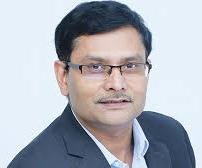
\includegraphics[scale=2.5]{src/Figures/authors/aloknath.png}} & 

\centerline{\large\bf Aloknath De}

 \bigskip
 Dr. Aloknath De is Chief Technology Officer of Samsung R\&D Institute India and also Senior VP for ‘Digital Media and Communication’ activities in Bangalore. Dr. De has more than twenty-five years of industrial and research experiences including the most recent one in ST-Ericsson where he was Director and Country Manager. He holds B.Tech. from Indian Institute of Technology (IIT), Kharagpur; M.E. from Indian Institute of Science (IISc), Bangalore; and Ph.D. from McGill University, Montreal. He is a recipient of ‘Alexander Graham Bell Prize’ in Canada and received IETE Memorial Awards in India. Dr. De has served as an Adjunct Professor with IIT-Delhi and also as an AICTE-INAE Distinguished Visiting Professor
with IIT-Roorkee. He is a senior member of IEEE, and fellows of IE, IETE and INAE.\\
&\\ 
\clineB{1-2}{2.5}
\end{tabular}


%~ \vskip 1cm

%~ \begin{figure}[H]
%~ \centering
%~ 
\includegraphics[scale=.15]{src/Figures/QR-codes/qr-code_a-review-on-3gpp.png}

%~ \medskip

%~ {\large\sf Access this article on the Web}
%~ \end{figure}
